\documentclass{article}
\usepackage[utf8]{inputenc}
\usepackage{listings}
\usepackage[italian]{babel}
\usepackage{subfiles}
\usepackage{enumerate}
\usepackage{color}
\textwidth=450pt\oddsidemargin=0pt
\usepackage{graphicx}
\usepackage{caption}
\usepackage{subcaption}
\usepackage{wrapfig}
\usepackage{tikz}
\usepackage[colorlinks=true,linkcolor=black,urlcolor=black, citecolor=black]{hyperref}
\usepackage{amsmath}
\usepackage{amsthm}
\usepackage{amssymb}
\usepackage{mathtools}
\usepackage{subfiles}
\usepackage{comment}
\usepackage{float}
\usepackage{enumerate}
\usepackage{appendix}
\usepackage[style=numeric, backend=biber, sorting=nty]{biblatex}
\usepackage{chngcntr}
\usepackage{fancyhdr}

\newcommand{\bb}[1]{\textbf{#1}}
\newcommand{\ii}[1]{\textit{#1}}

\title{Struttura e Risultati}
\author{ Lamma Tommaso}
\date{Luglio 2021}

\begin{document}

\maketitle

\tableofcontents

\newpage

\section{Struttura del Codice in C++}

    \subsection{Classi}
        \paragraph{car.cpp}
            La classe \bb{Car} ha come attributi privati:
            \begin{itemize}
                \item \bb{short int \_steps}, ovvero il numero di volte in cui l'automobile si è spostata effettivamente nel reticolo.
                \item \bb{short int \_stops}, ovvero il numero di volte in cui l'automobile ha dovuto fermasi a causa del traffico.
                \item \bb{short int \_offset}, ovvero la posizione all'interno della strada.
                \item \bb{bool \_at\_destination}, che diventa vera quando l'auto giunge a destinazione.
                \item \bb{short int \_delay}, ovvero un ritardo nella partenza, poiché dato che tutte le auto
                    sono generate con offset nullo, per evitare sovrapposizioni devono partire una alla volta.
            \end{itemize}
        \paragraph{road.cpp}
            La classe \bb{Road} ha come attributi privati:
            \begin{itemize}
                \item \bb{short int \_car\_number}, ovvero il numero di auto presenti nella strada.
                \item \bb{short int \_road\_length}, ovvero la lunghezza della strada.
                \item \bb{short int \_width}, ovvero il numero di corsie della strada, uguale a 1 nelle strade che fanno parte di un doppio senso,
                    e variabile per i sensi unici.
                \item \bb{static *}, dove * si riferisce ai parametri statistici delle strade spiegati nella sezione precedente, messi come
                    \ii{static} per migliorare l'uso della memoria.
            \end{itemize}
        \paragraph{node.cpp}
            La classe \bb{Node} ha come unico attributo privato:
            \begin{itemize}
                \item \bb{short int \_index}, ovvero l'etichetta del nodo.
            \end{itemize}
        \paragraph{city.cpp}
            La classe \bb{City} ha come attributi privati:
            \begin{itemize}
                \item \bb{Node** \_path} e \bb{short int** \_distance}, che servono a determinare il percorso più efficiente tra due nodi.
                \item \bb{void \_floyd\_warshall}, che dalla matrice di adiacenza determina i due attributi precedenti.
                \item \bb{Node* \_node\_set}, ovvero l'insieme dei nodi della città.
                \item \bb{Road** \_adj\_matrix}, ovvero la matrice di adiacenza del grafo diretto che rappresenta la città.
                \item \bb{short int \_n\_rows} e \bb{short int \_n\_coloumns}, che sono ripettivamente il numero di righe e colonne della griglia che è la città.
                \item \bb{float \_oneway\_fraction}, ovvero un parametro che in generazione determina la probabilità di avere sensi unici,
                    tale parametro può essere diverso dall'effettiva frazione, soprattutto per città piccole, ma nei grafici riportiamo sempre la 
                    frazione effettiva invece che questo parametro.
            \end{itemize}
        \paragraph{simulator.cpp}
            La classe \bb{Simulator} ha necessita di due \ii{struct} aggiuntive:
            \begin{enumerate}
                \item \bb{Car\_Info}, che ha come attributi il percorso di un'auto, il nodo appena passato, e un puntatore a macchina per gestire i dati di traffico.
                \item \bb{Result}, che contiene le statistiche rilevanti della simulazione.
            \end{enumerate}
            Inoltre ha come attributi privati:
            \begin{itemize}
                \item \bb{std::vector$\langle$Car\_Info$\rangle$ \_car\_vector}, tale vettore è usato per associare ad ogni auto un percorso ed un nodo tramite l'indice 
                    all'interno del std::vector. Tale implementazione è necessaria in quanto a ogni iterazione viene chiamato un \ii{sort} che permette di 
                    muovere prima le auto con offset maggiore, riducendo il numero di iterazioni necessarie.
                \item \bb{Result \_result}, ovvero i risulati della simulazione.
                \item \bb{short int \_cars\_at\_destination}, fa proseguire la simulazione finché non eguaglia il numero di automobili generate.
                \item \bb{City \_city}, ovvero la città su cui viene effettuata la simulazione.
                \item \bb{short int \_car\_number}, ovvero il numero di auto generate.
                \item \bb{void \_mv\_car(int car\_index)}, che gestisce tutti i controlli del traffico e muove le automobili.
                    Tale metodo prende la posizione della macchina in \_car\_vector, poiché senza di esso non sappiamo nulla della macchina.
                \item other useful inline functions.
            \end{itemize}
        \paragraph{js\_interface.cpp} 
            La classe \ii{js\_interface.cpp} serve alla grafica, scritta in javascript per interagire con il codice della simulazione in C++.
        \paragraph{numpy\_parser.cpp}
        La classe \ii{numpy\_parser.cpp} serve a creare file python con numpy.array leggibili dalla libreria di graficamento \ii{matplotlib}, 
            a partire da std::vector del C++.
    
    \subsection{Considerazioni}
        La scelta di avere oggetti che essenzialmente sono solo uno o due interi (short) è dovuta ad alcuni problemi nella creazione della matrice di adiacenza.
        Infatti usare strutture più ingombranti causava errori di segmentazione durante la creazione della città, probabilmente dovuto al fatto che la memoria
        occupata dalla matrice di adiacenza eccedeva quella riservata al programma.
        La scelta di avere classi non interagenti che possono interagire solo tramite la classe \ii{Simulator}, è dovuta a problemi di ricorsività
        emersi durante le prime versioni del programma.

\section{Risultato delle Simulazioni}
    
    \subsection{Car Increment Simulation}
        Le simulazioni mostrano che fissata la città, l'indice di traffico aumenta all'aumentare delle automobili
        e tende a 1 per il numero di automobili che tende a zero. Ovviamente tale simulazione non avrebbe senso, per ciò 
        partiamo da almeno 1 macchina nella città, l'indice di traffico che emerge dalla simulazione con una sola macchina
        sarà 1 poiché non può esistere un rallentamento.
        In Fig. \ref{fig:3} è riportato l'esito di circa 70 simulazioni che incrementano di 1 il numero di automobili da 1 a 2000.
        Ciò è stato fatto su una città $5 \times 5$ senza senzi univi per verificare che effettivamente il traffico aumentasse
        all'aumentare delle auto.

        \begin{figure}[H]
            \begin{minipage}{.5\textwidth}
                \centering
                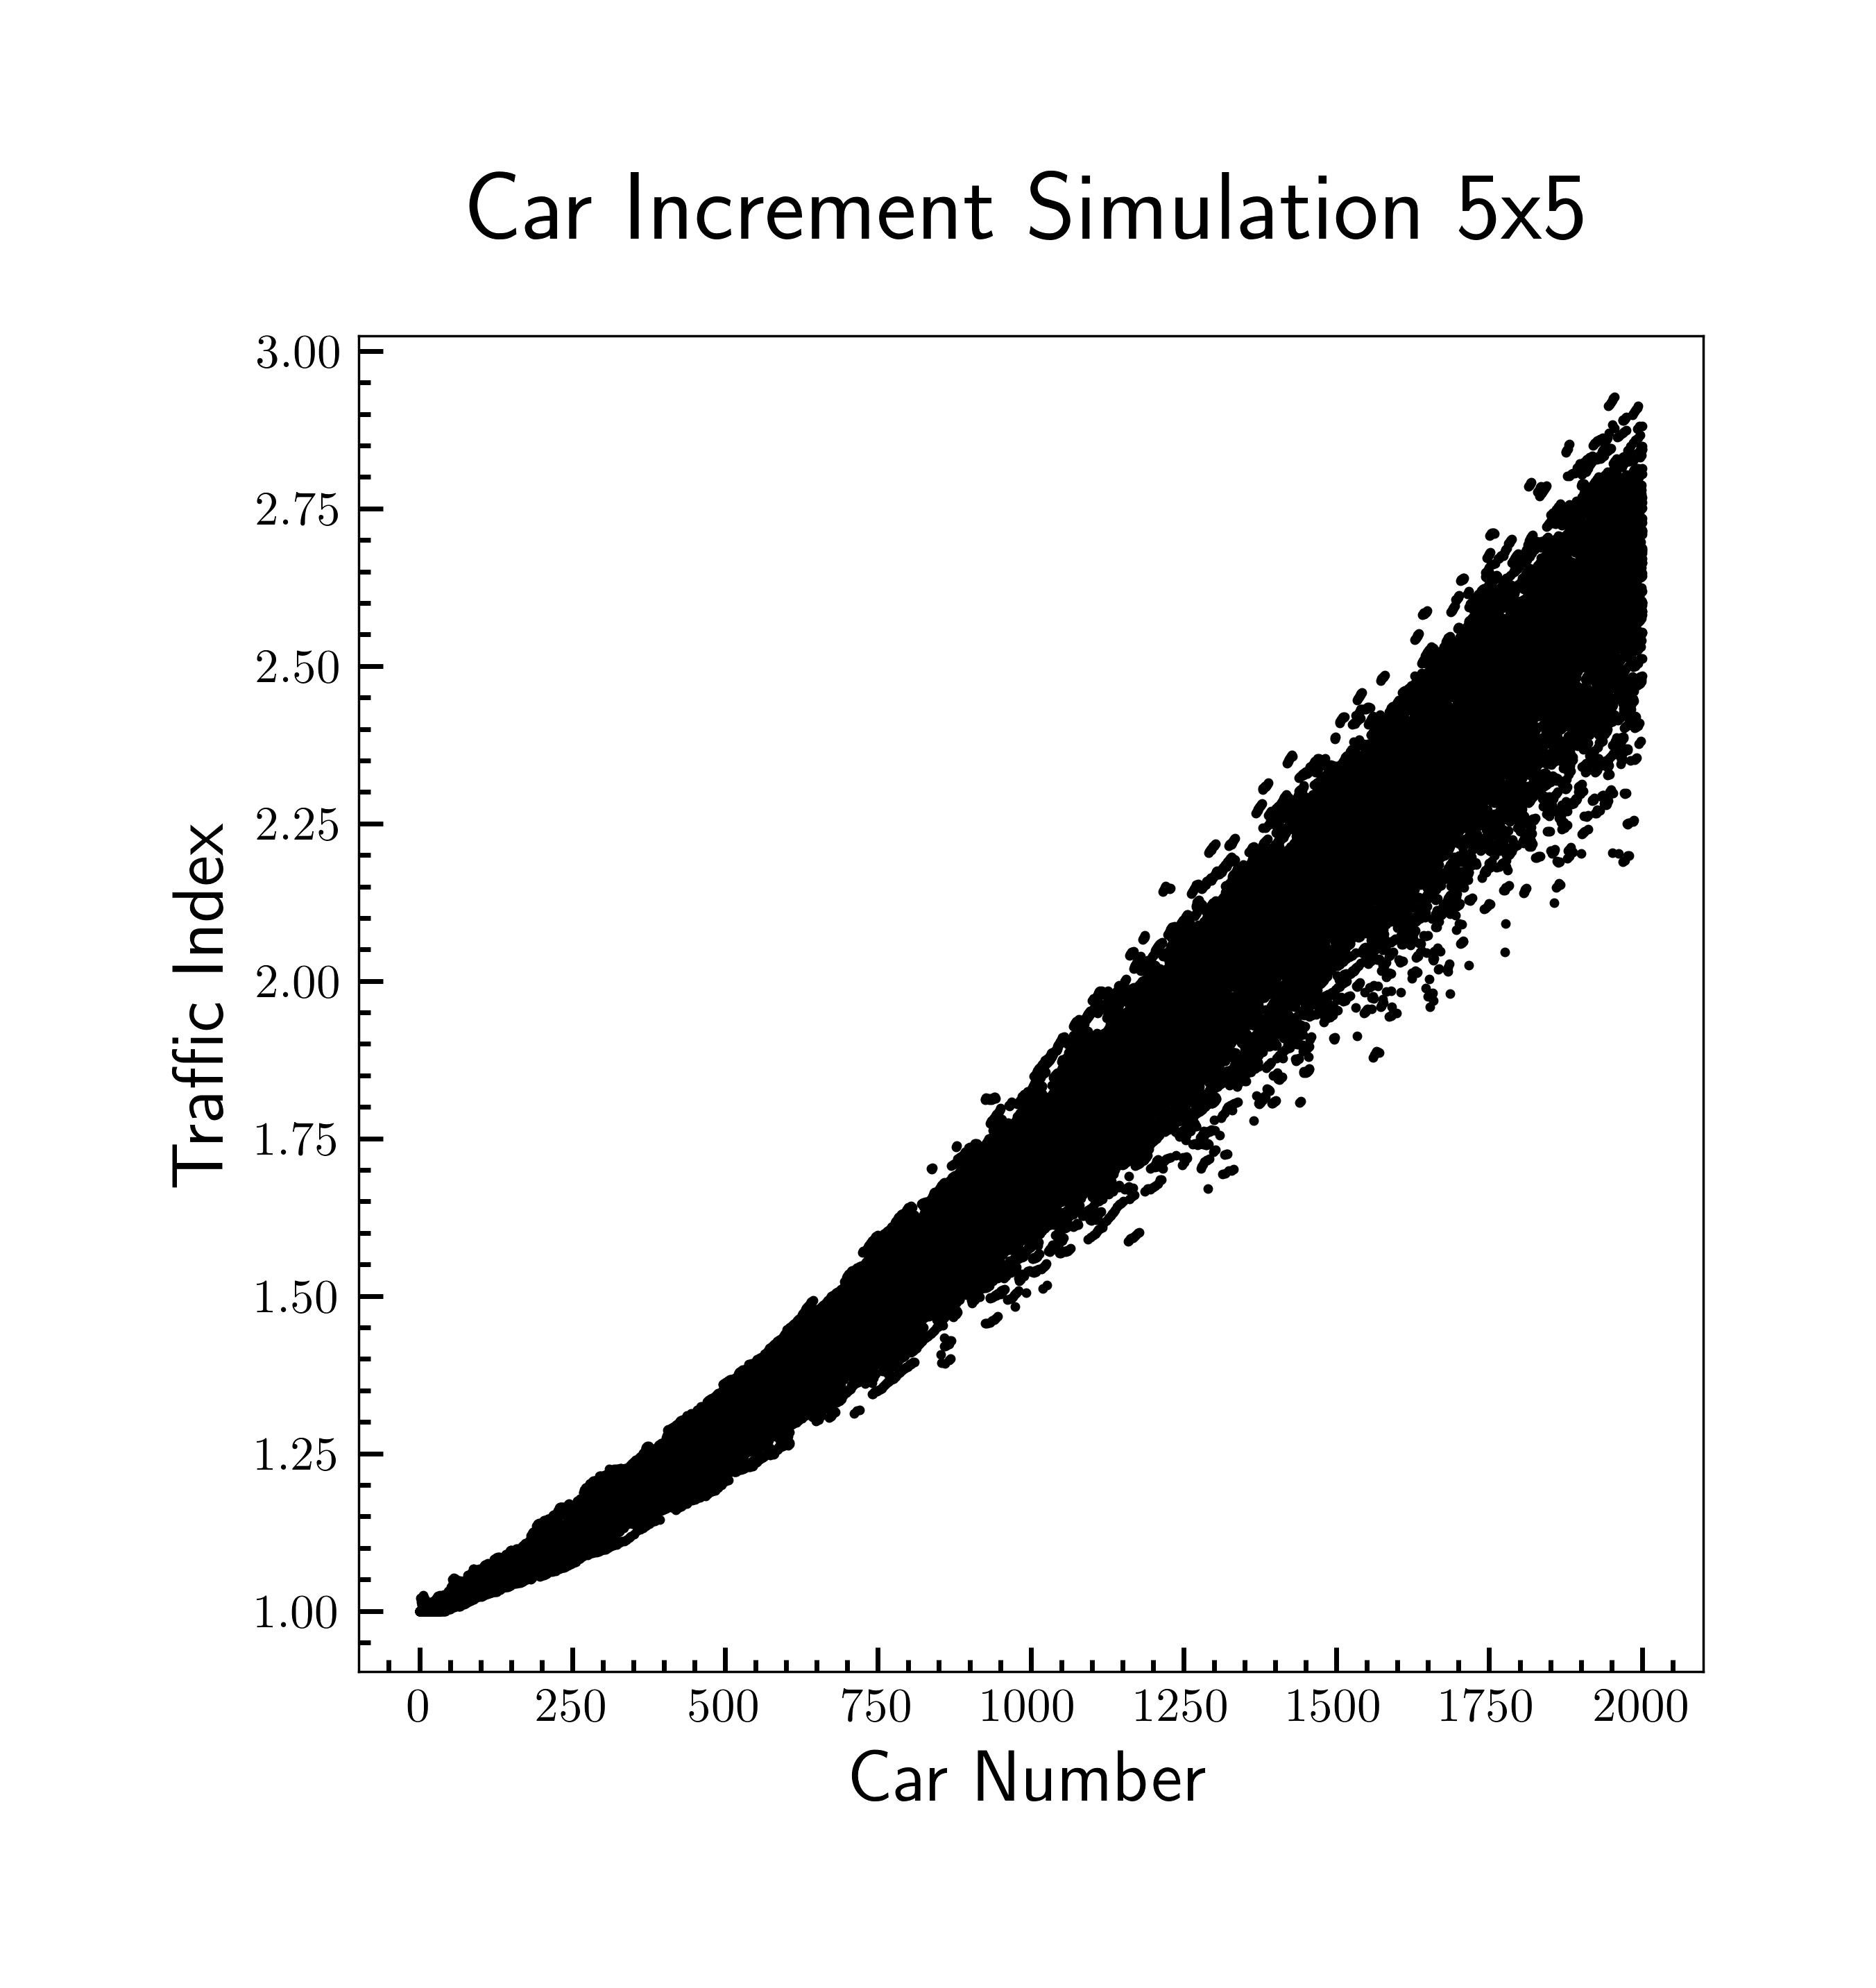
\includegraphics[width=8cm, height=8cm]{car_increment5x5.png}
                \caption{Car Increment Simulation\\ su una città $5 \times 5$ senza sensi unici.}
                \label{fig:3}
            \end{minipage}
            \begin{minipage}{.5\textwidth}
                \centering
                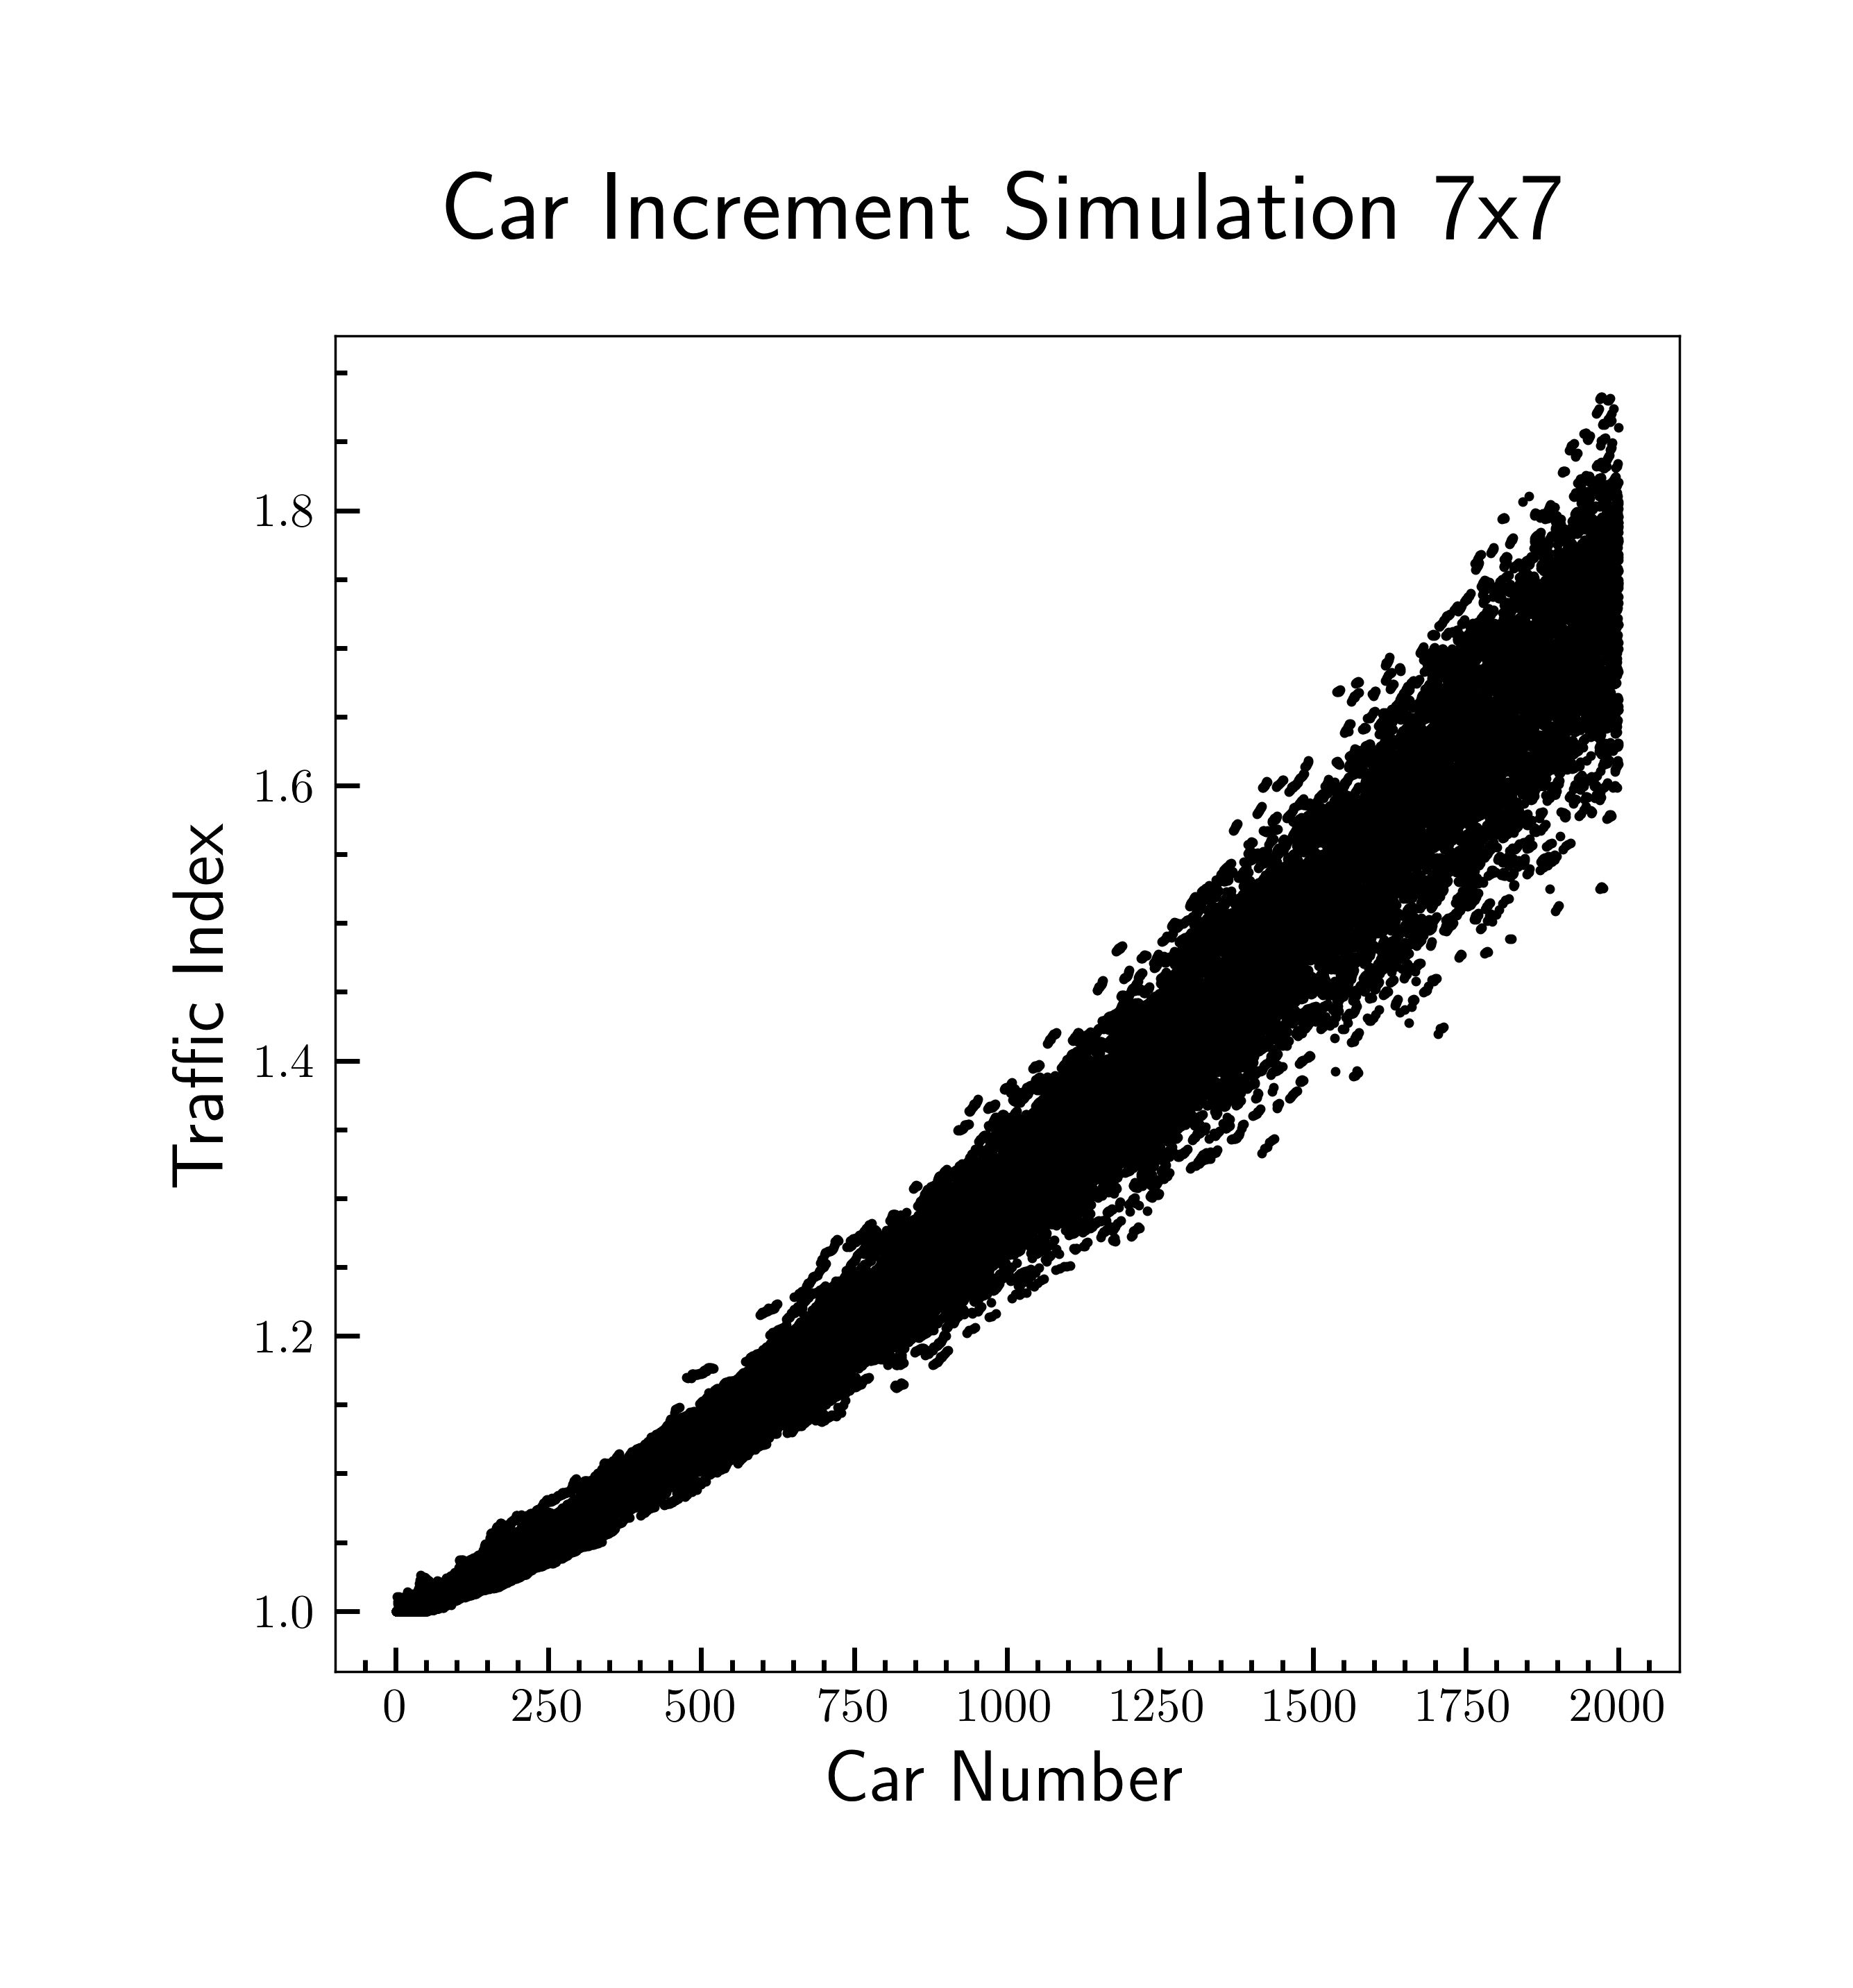
\includegraphics[width=8cm, height=8cm]{car_increment7x7.png}
                \caption{Car Increment Simulation su una città $7 \times 7$ senza sensi unici.}
                \label{fig:4}
            \end{minipage}
        \end{figure}

        Per entrambe queste simulazioni si è usata la seguente statistica delle strade:
        \begin{itemize}
            \item media della lunghezza : 20
            \item deviazione standard della lunghezza : 10
            \item lunghezza massima : 30
            \item lunghezza minima : 10
        \end{itemize}

        Un' osservazione interessante che può essere fatta a partire da queste statistiche è che su città rispettivamente
        $5 \times 5$ e $7 \times 7$ generano una superficie stradale media data da $20 \times 5 \times 4 \times 2 = 800$ e
        $20 \times 7 \times 6 \times 2 = 1680$. Data questa considerazione, notiamo che quando il numero di auto è confrontabile con 
        la superficie media nelle due simulazioni l'indice di traffico si trova sempre attorno a 1.5.
        Perciò possiamo pensare che senza ulteriori modifiche topologiche, l'indice di traffico su una città a griglia
        senza sensi unici dipenda esclusivamente dalla densità di automobili.

        Il fatto che a densità uguale a 1 il programma non si blocchi è dovuto ad un controllo che fa partire le auto con diversi ritardi,
        quindi non tutte le auto indicate da car number saranno nella città contemporaneamente.
        Da questa anilisi preliminare possiamo concludere che il traffico emerge dal nostro modello e dipende dalla densità di auto,
        come suggerito da tutti i modelli di traffico esistenti.

    \subsection{Oneway Increment Simulation}
        Per vedere se aumentare il numero di sensi unici è in alcuni casi conveniente, abbiamo fatto una simulazione aumentando la frazione di sensi unici 
        fissate 1000 automobili utilizzando le stesse statistiche stradali della sezione precedente. Tale simulazione è stata eseguita per diverse larghezze dei sensi unici, ovvero una, due e tre corsie.
        L'incremento del parametro di generazione \_oneway\_fraction è stato scelto essere 0.001.
        In Fig. \ref{fig:5} è mostrata la simulazione con sesi unici larghi una sola corsia che, causando una riduzione della superficie media, è chiaramente sconveniente.
        
        \begin{figure}[H]
            \centering
            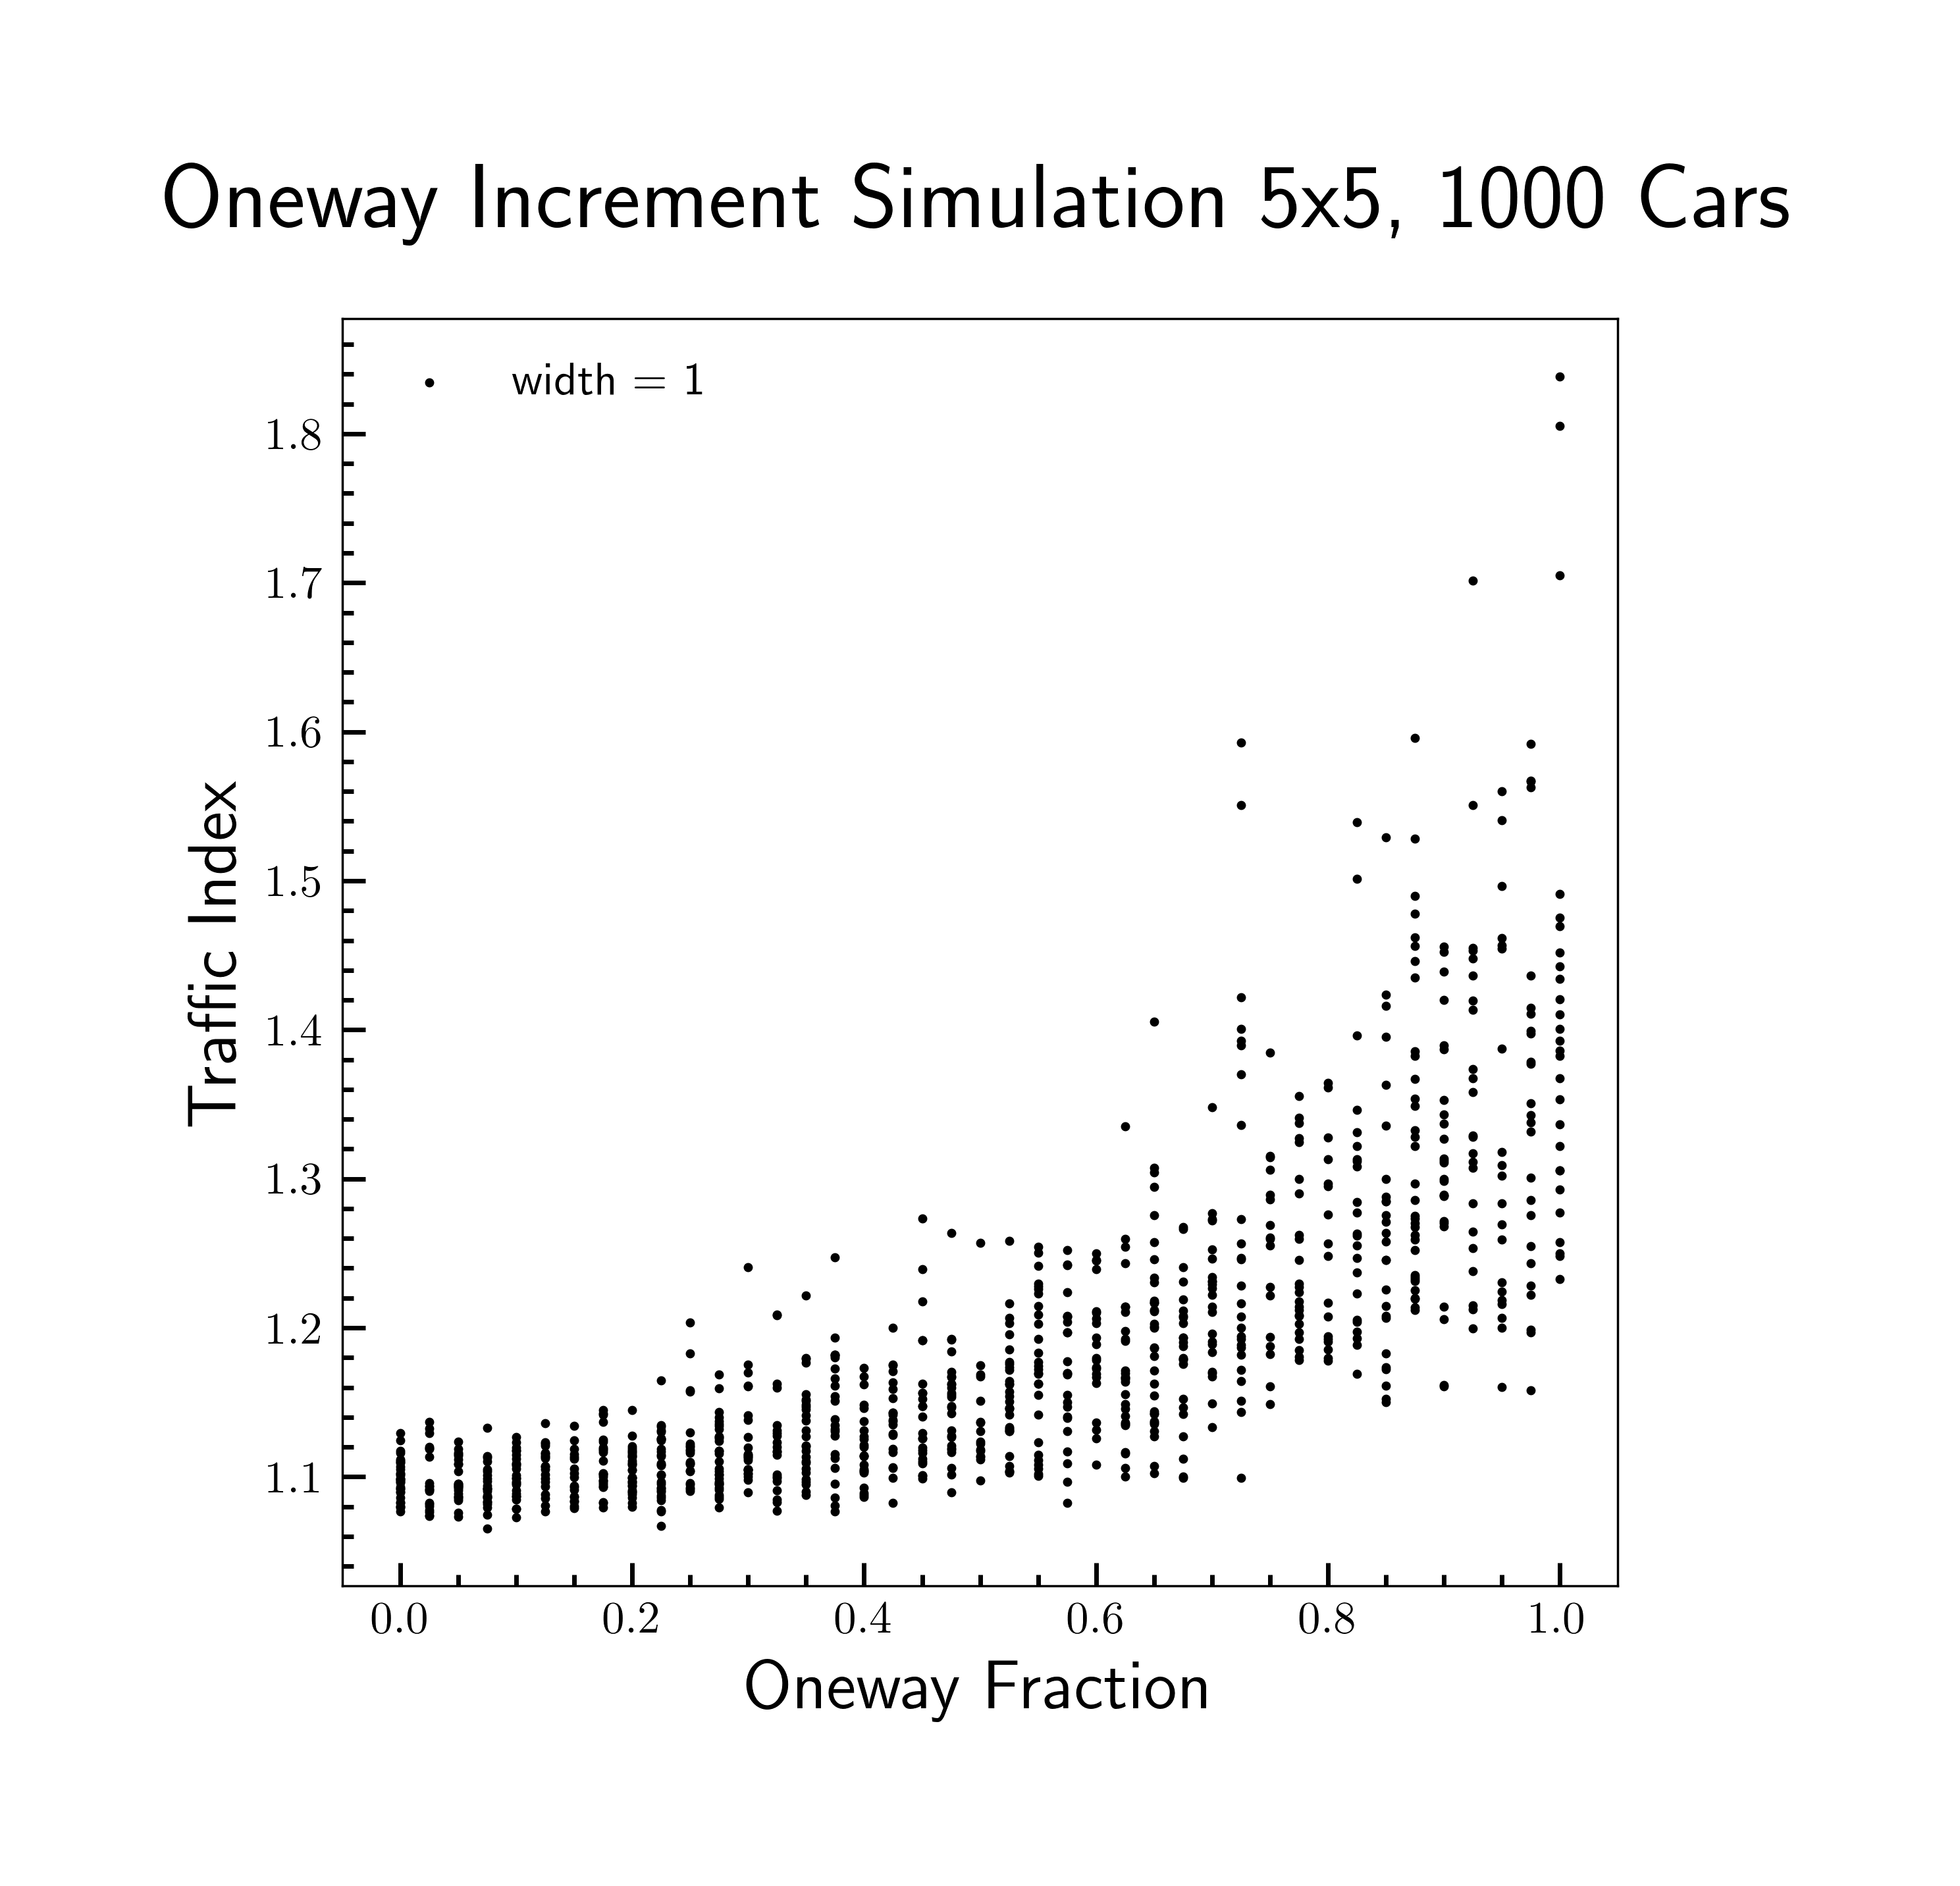
\includegraphics[width=10cm, height=10cm]{oneway_increment_1.png}  
            \caption{Oneway Increment Simulation su una città $5 \times 5$, con larghezza uguale a uno.}
            \label{fig:5}
        \end{figure}

        Da questo grafico possiamo notare che il traffico aumenterà sempre aumentando i sensi unici a meno della fluttuazione dovuta
        al posizionamento dei sensi unici nella città. Infatti si può notare che la sezione verticale della fascia nera del grafico si allarga
        andando verso destra. Ciò significa che in città con tanti sensi unici l'indice di traffico dipenderà molto dal modo in cui essi sono disposti
        e non solo dalla frazione.

        In Fig. \ref{fig:6} e in Fig. \ref{fig:7} è mostrata la stessa simulazione con sensi unici rispettivamente a due e tre corsie.

        \begin{figure}[H]
            \begin{minipage}{.5\textwidth}
                \centering
                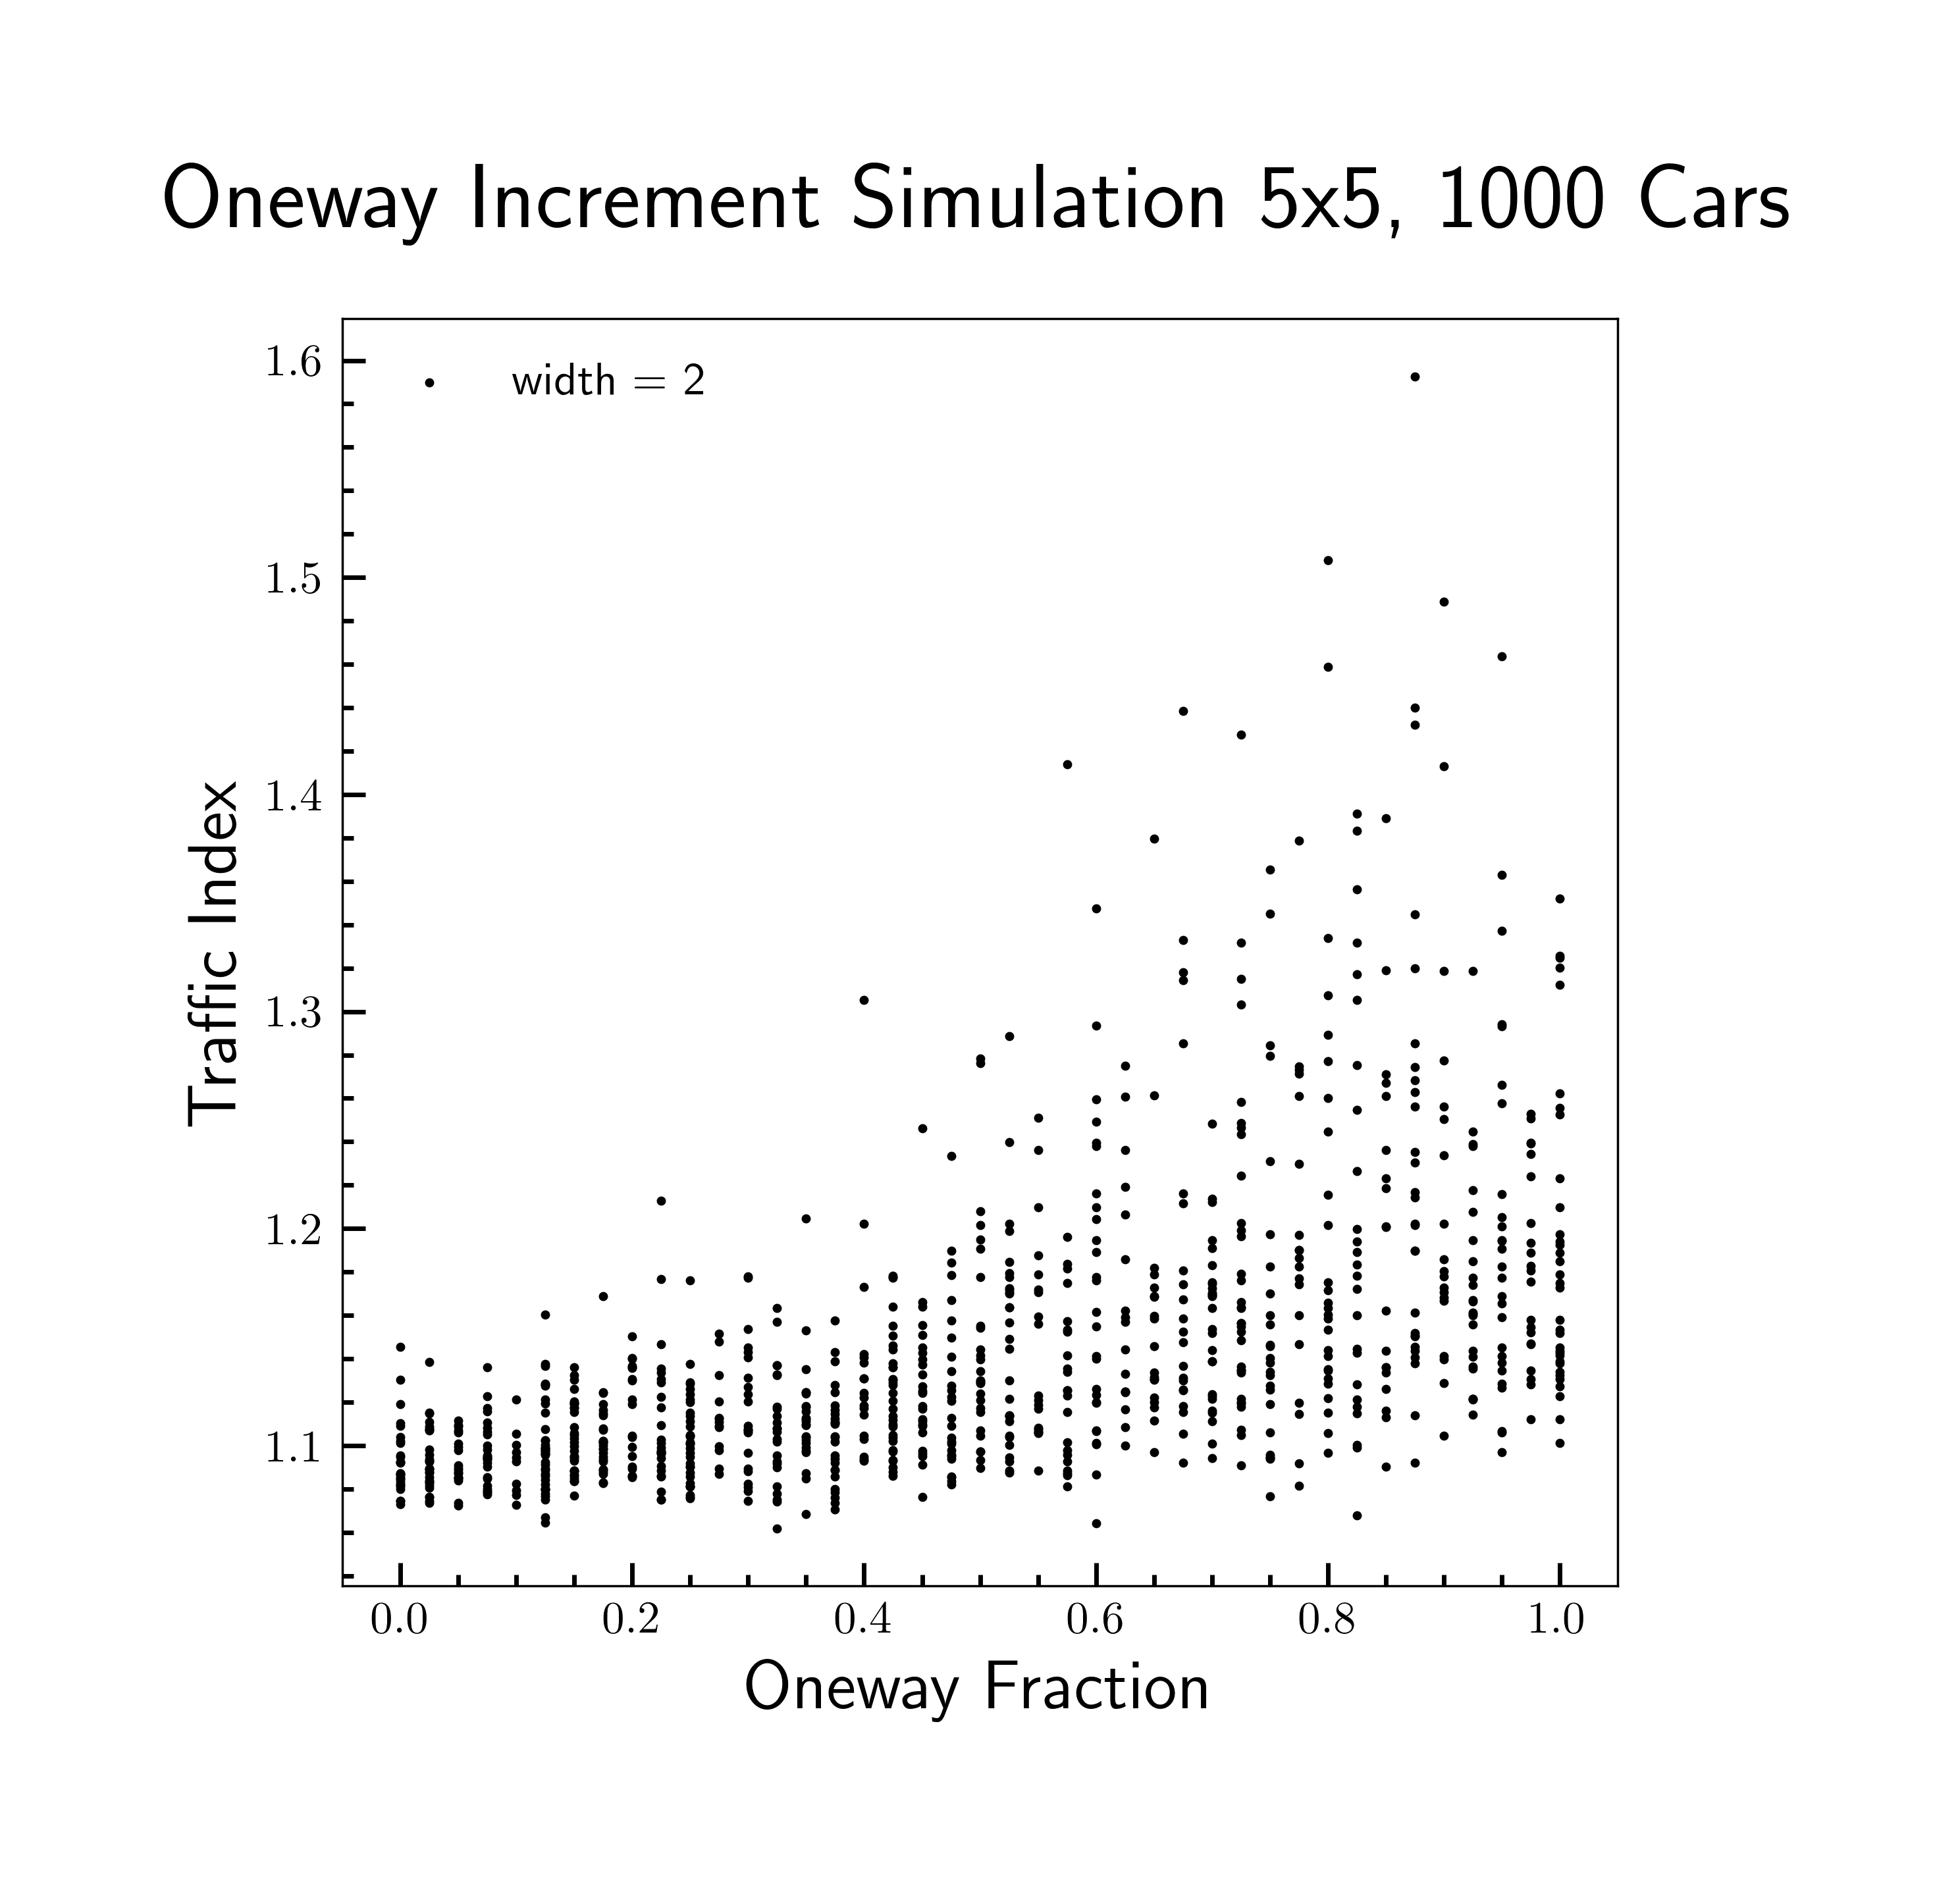
\includegraphics[width=8cm, height=8cm]{oneway_increment_2.png}  
                \caption{Oneway Increment Simulation su\\ una città $5 \times 5$, con larghezza uguale a due.}
                \label{fig:6}
            \end{minipage}
            \begin{minipage}{.5\textwidth}
                \centering
                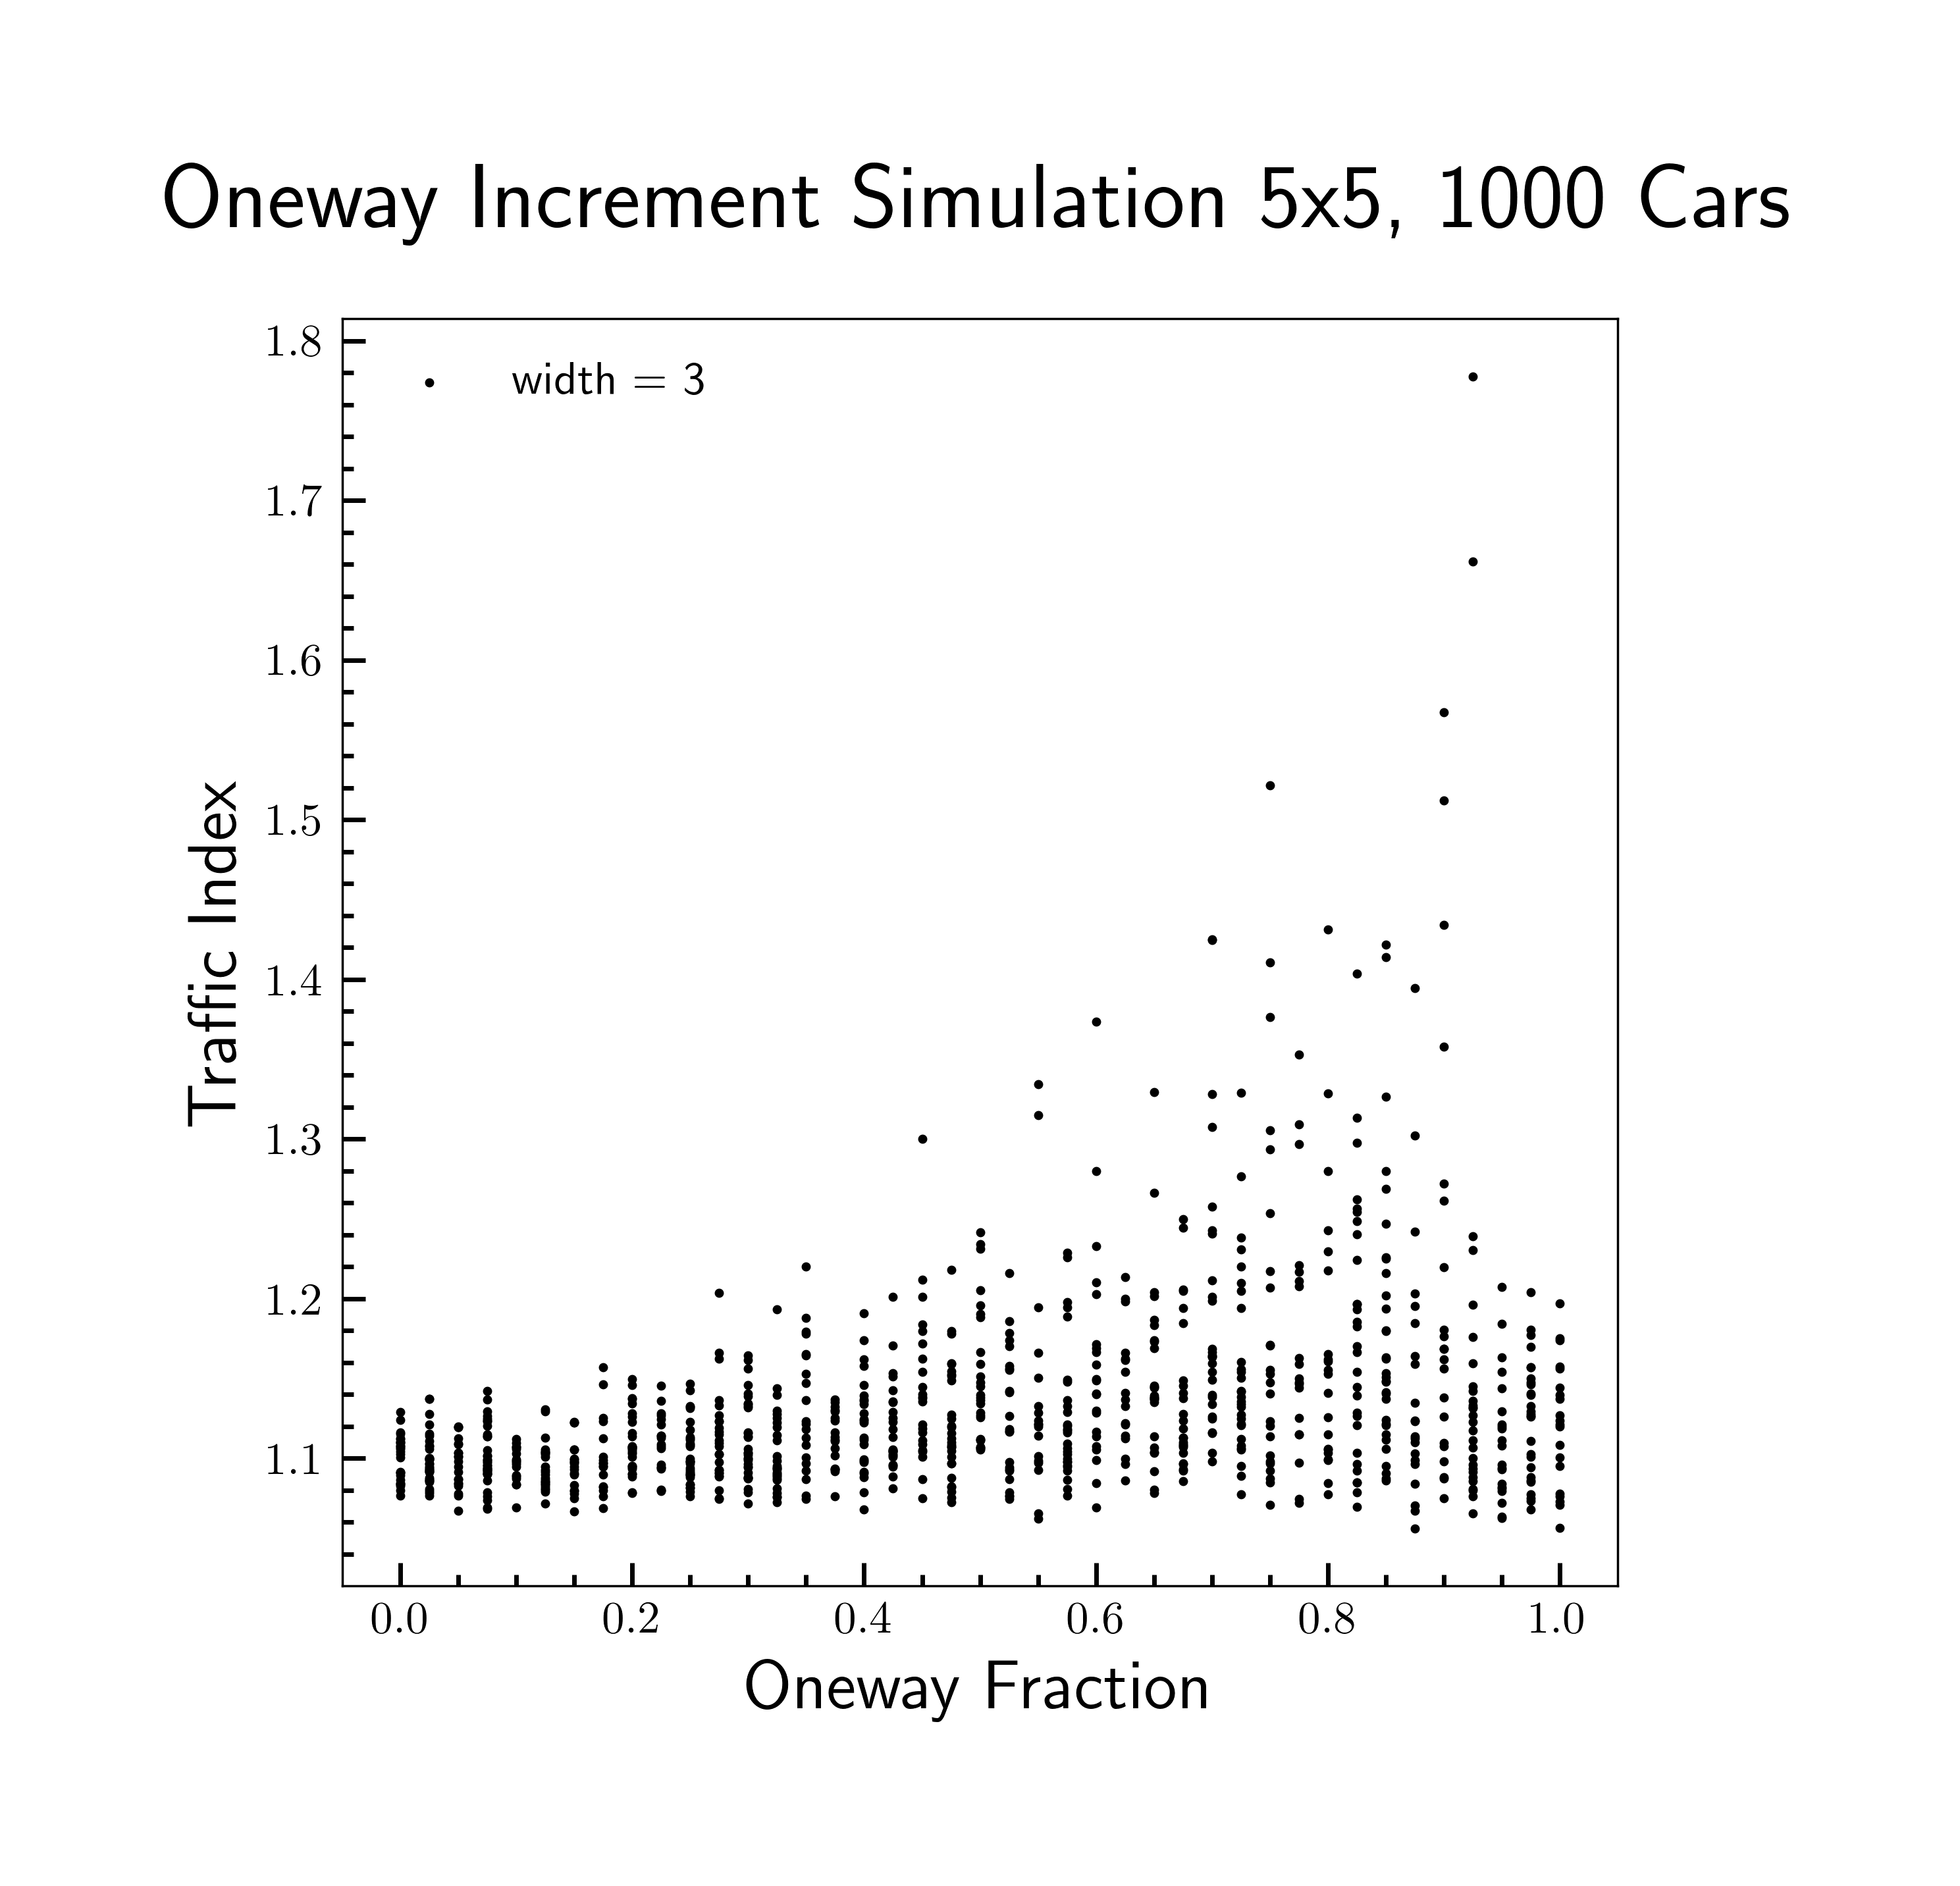
\includegraphics[width=8cm, height=8cm]{oneway_increment_3.png}  
                \caption{Oneway Increment Simulation su una città $5 \times 5$, con larghezza uguale a tre.}
                \label{fig:7}
            \end{minipage}
        \end{figure}

        In Fig. \ref{fig:6} a differenza del grafico precedente, notiamo che per un'alta frazione di sensi unici si hanno comunque città
        con un indice di traffico relativamente basso. Quindi possiamo dire che esiste un modo per disporre molti sensi unici a molte corsie per
        ridurre l'indice di traffico. Tuttavia tale fatto potrebbe anche essere dovuto all'aumento della superficie media della città all'aumentare dei 
        sensi unici, che perciò andrebbe a ridurre la densità di automobili riducendo l'indice di traffico.
        Tale effetto è maggiormente accentuato in Fig. \ref{fig:7}, mettendo sensi unici a tre corsie.\\
        \hfill\\

        In questi tre grafici l'effetto di "quantizzazione" della frazione di sensi unici è dovuto alle piccole dimensioni della città.
        Infatti il numero ridotto di strade, questa volta intese senza direzione, fa in modo che le frazioni di sensi unici non possano variare
        continuamente.

        \newpage

        Un'altra analisi che è stata fatta, approssimando linearmente gli esiti delle car increment simulation a diverse frazioni di sensi unici, consiste nel vedere
        come la pendenza di tali rette varia al variare dei sensi unici, il grafico è riportato in Fig. \ref{fig:8} mentre in Fig. \ref{fig:9} è riportata 
        una giustificazione grafica dell'approssimazione lineare. La pendenza di tali rette rappresenta la risposta della città all'aumentare della densità di 
        automobili.

        \begin{figure}[H]
            \begin{minipage}{.5\textwidth}
                \centering
                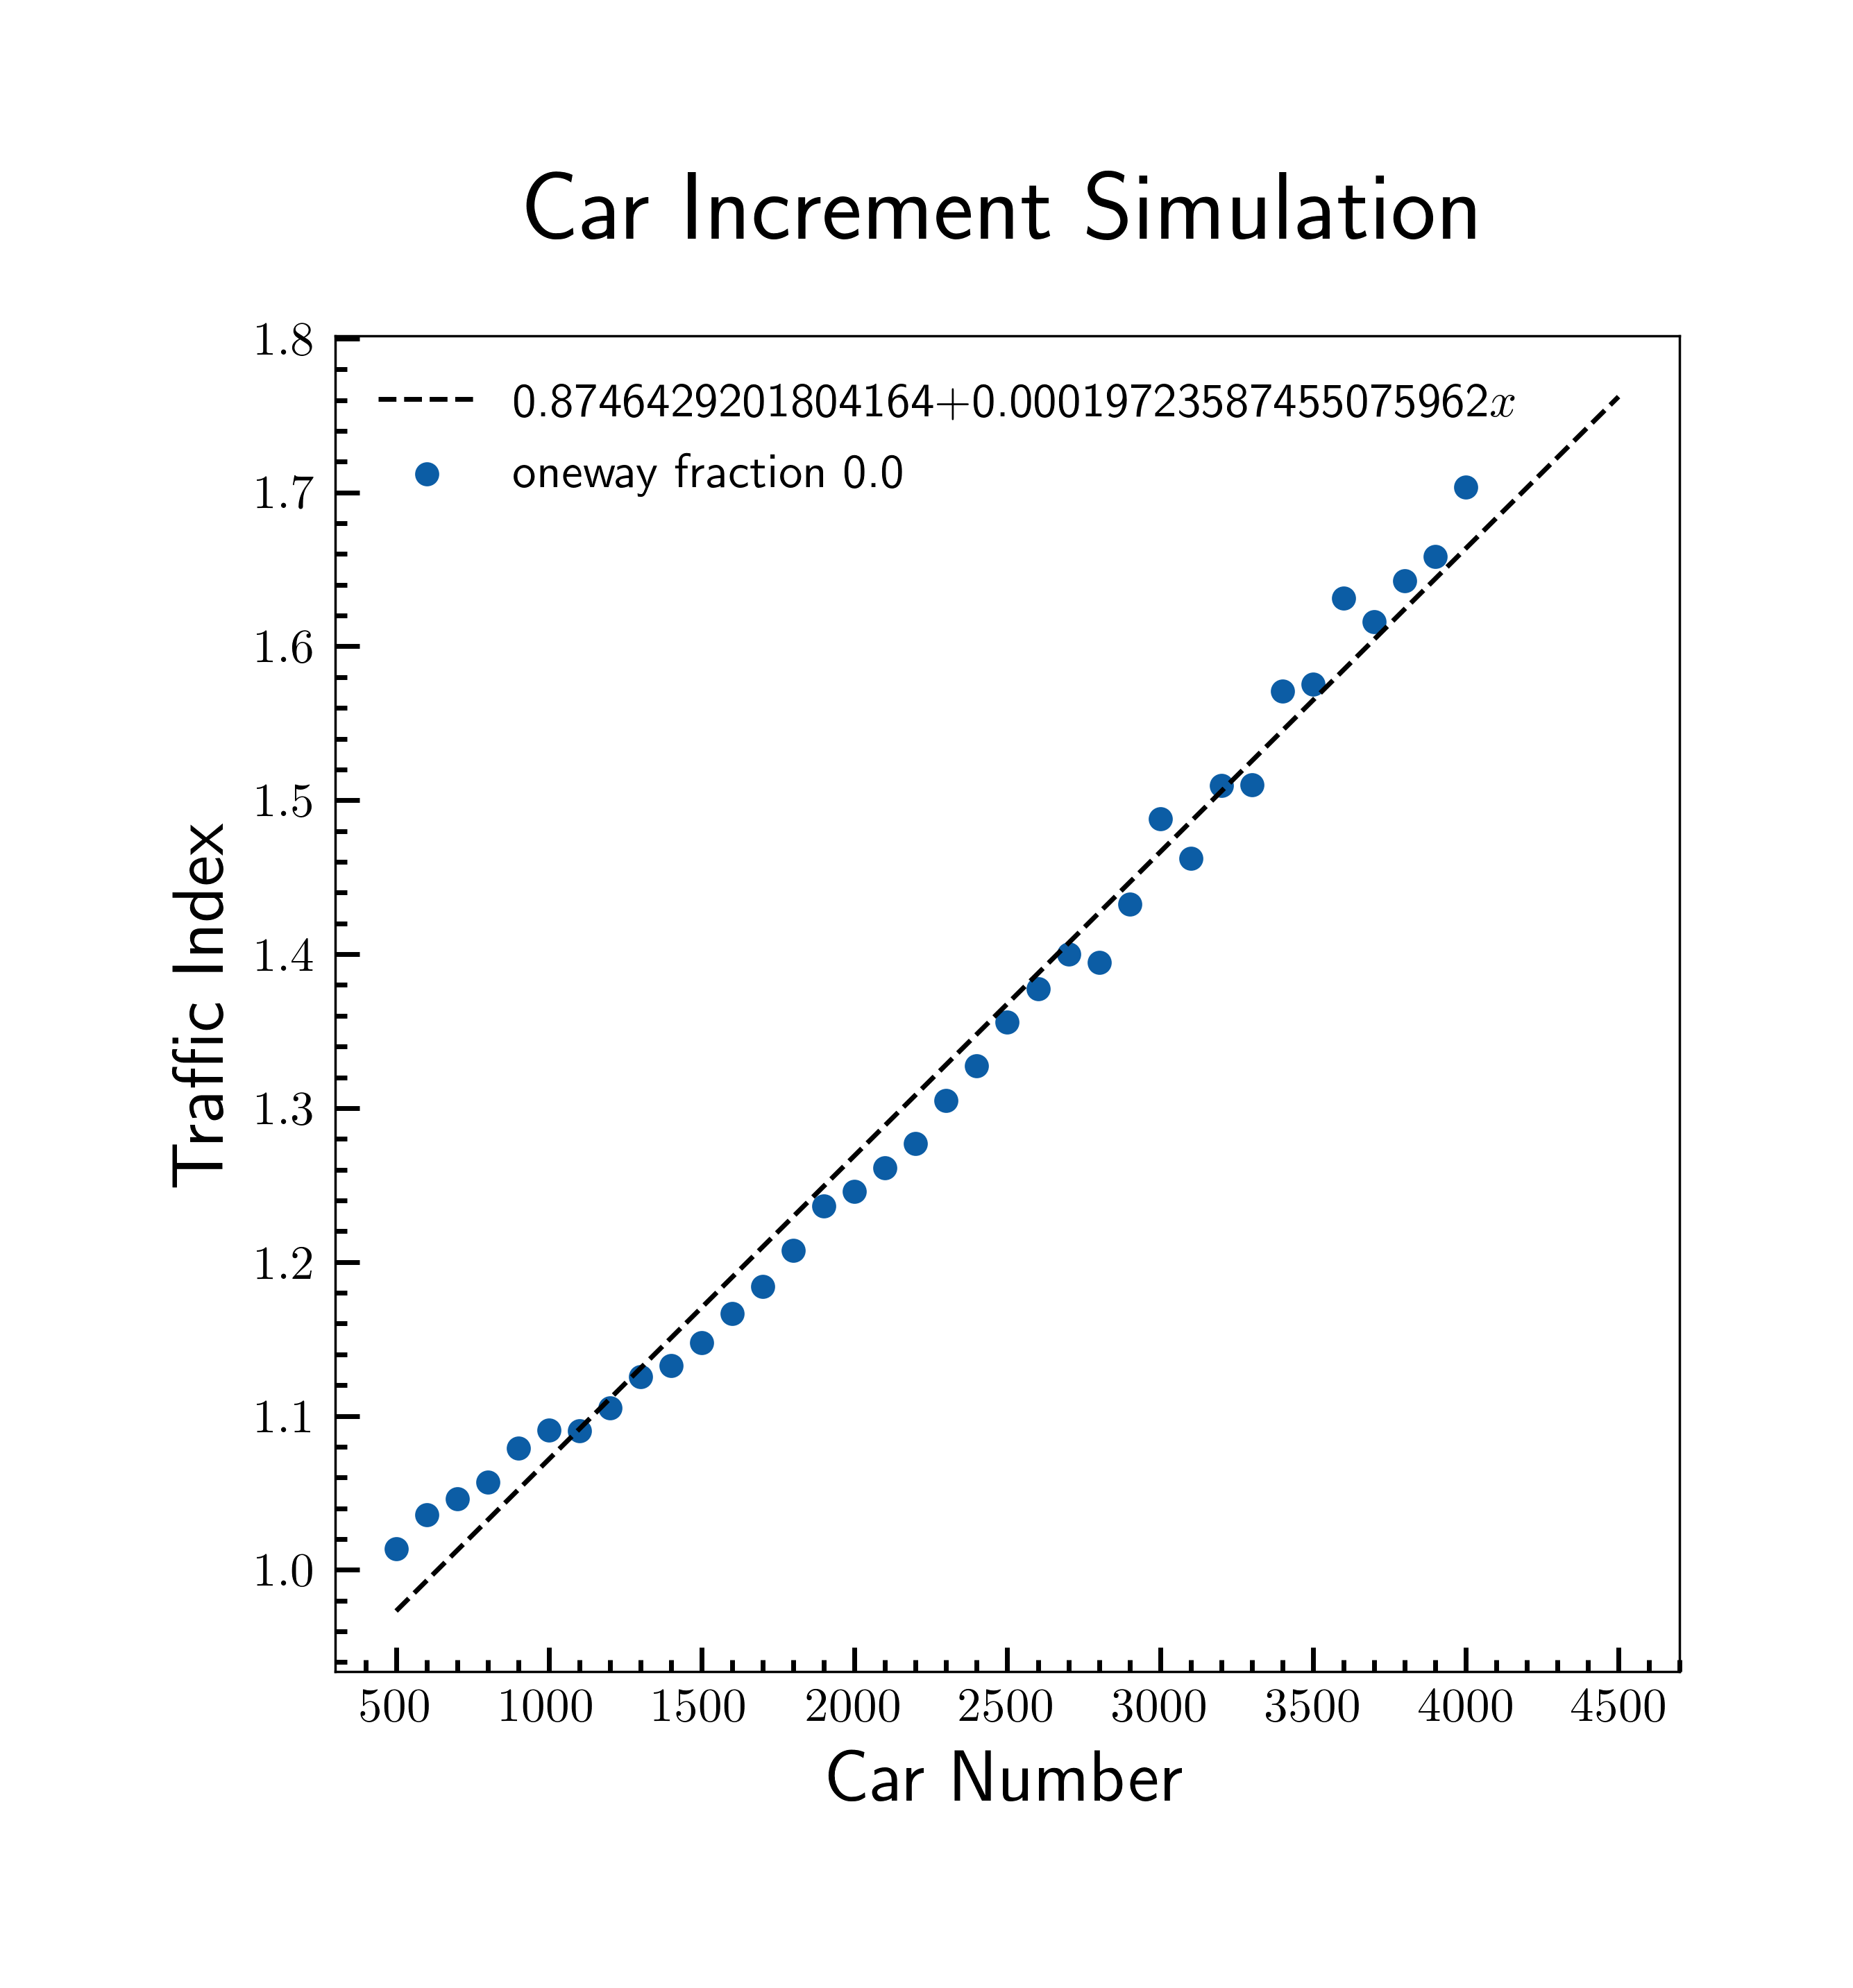
\includegraphics[width=8cm, height=8cm]{car_increment.png}
                \caption{Car Increment Simulation su\\ una città $10 \times 10$.}
                \label{fig:9}
            \end{minipage}
            \begin{minipage}{.5\textwidth}
                \centering
                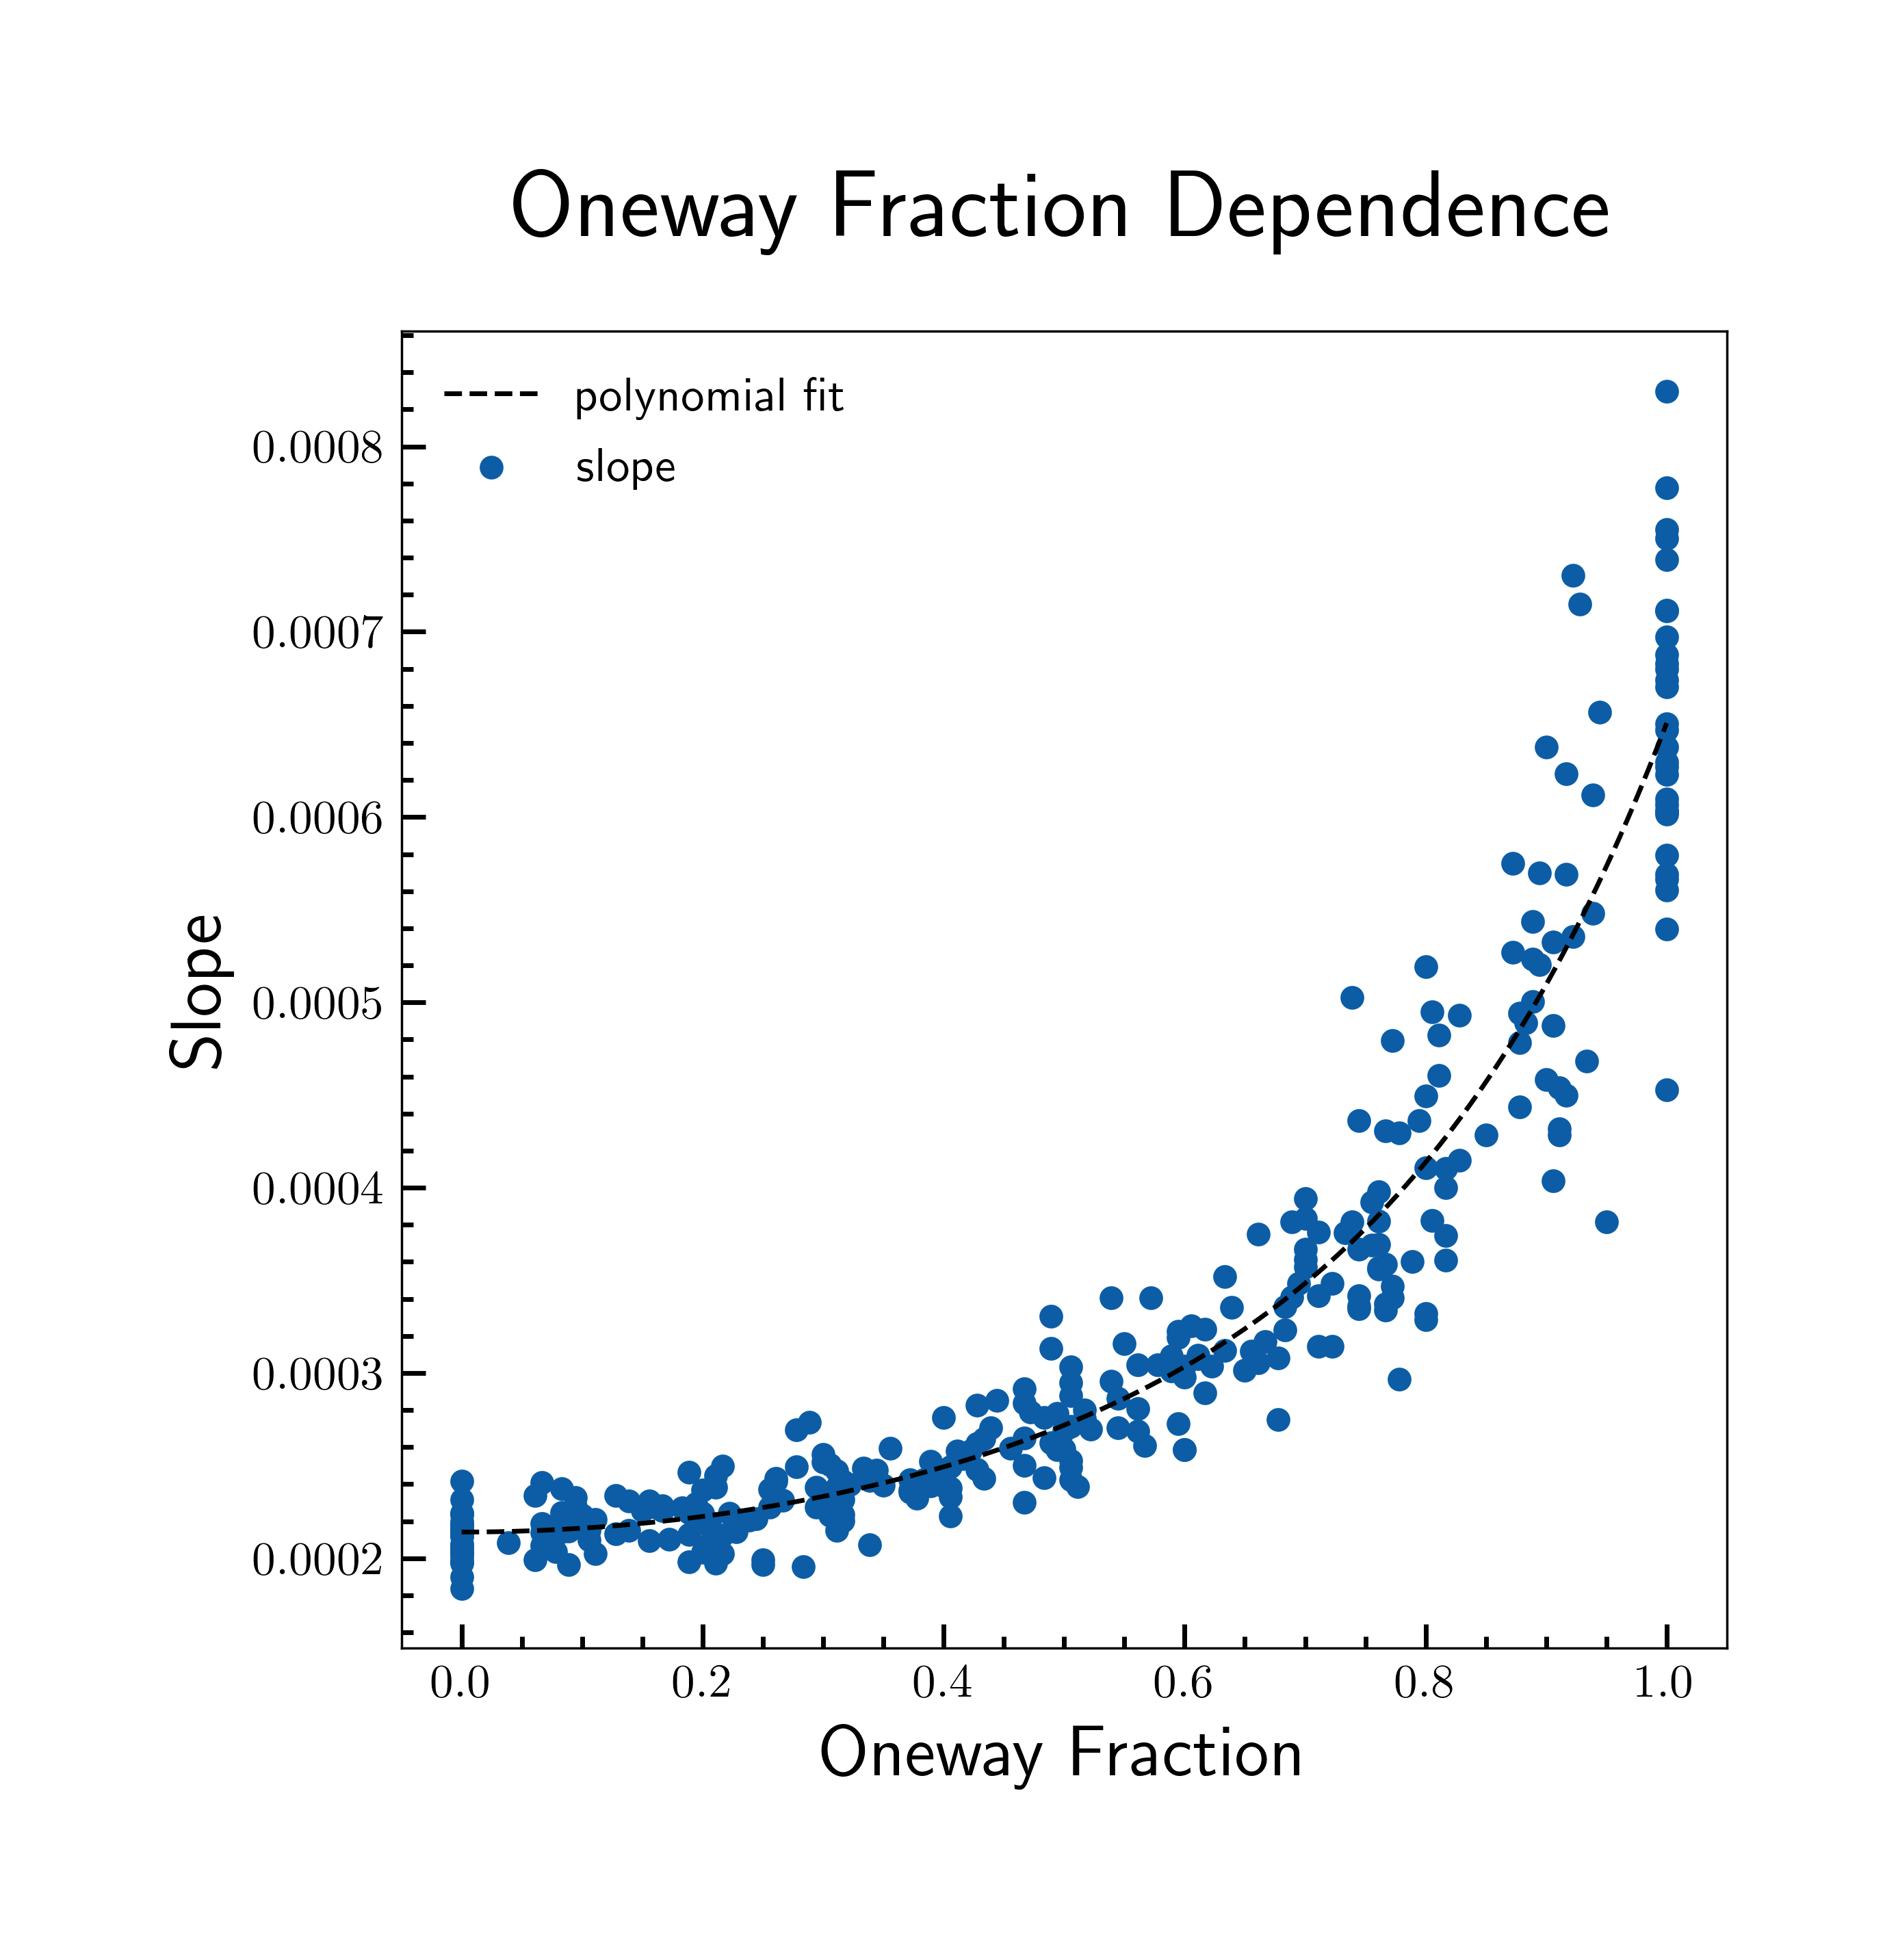
\includegraphics[width=8cm, height=8cm]{oneway_fraction_dependence.png}
                \caption{Variazione della pendenza della retta in funzione della frazione di sensi unici.}
                \label{fig:8}
            \end{minipage}
        \end{figure}

        Si è scelto un range lontano da $car\_number = 1$ dove l'indice di traffico non può seguire un andamento lineare per rispettare il limite ideale.
        Sulla stessa città $10 \times 10$ si sono eseguite varie car increment simulations variando i sensi unici, l'esito è riportato nella figura seguente\footnote{Si è scelto un fit polinomiale per semplicità.}.
        Da tale grafico è evidente che le città con un numero minore di sensi unici rispondono meglio all'aumentare della densità di automobili, come ci dovremmo
        aspettare da un modello di traffico.

        \newpage

        Un'ultima analisi è quella relativa ai tempi di esecuzione della oneway increment simulation su una città $10 \times 10$, il cui esito segue in Fig. \ref{fig:10}.

        \begin{figure}[H]
            \centering
            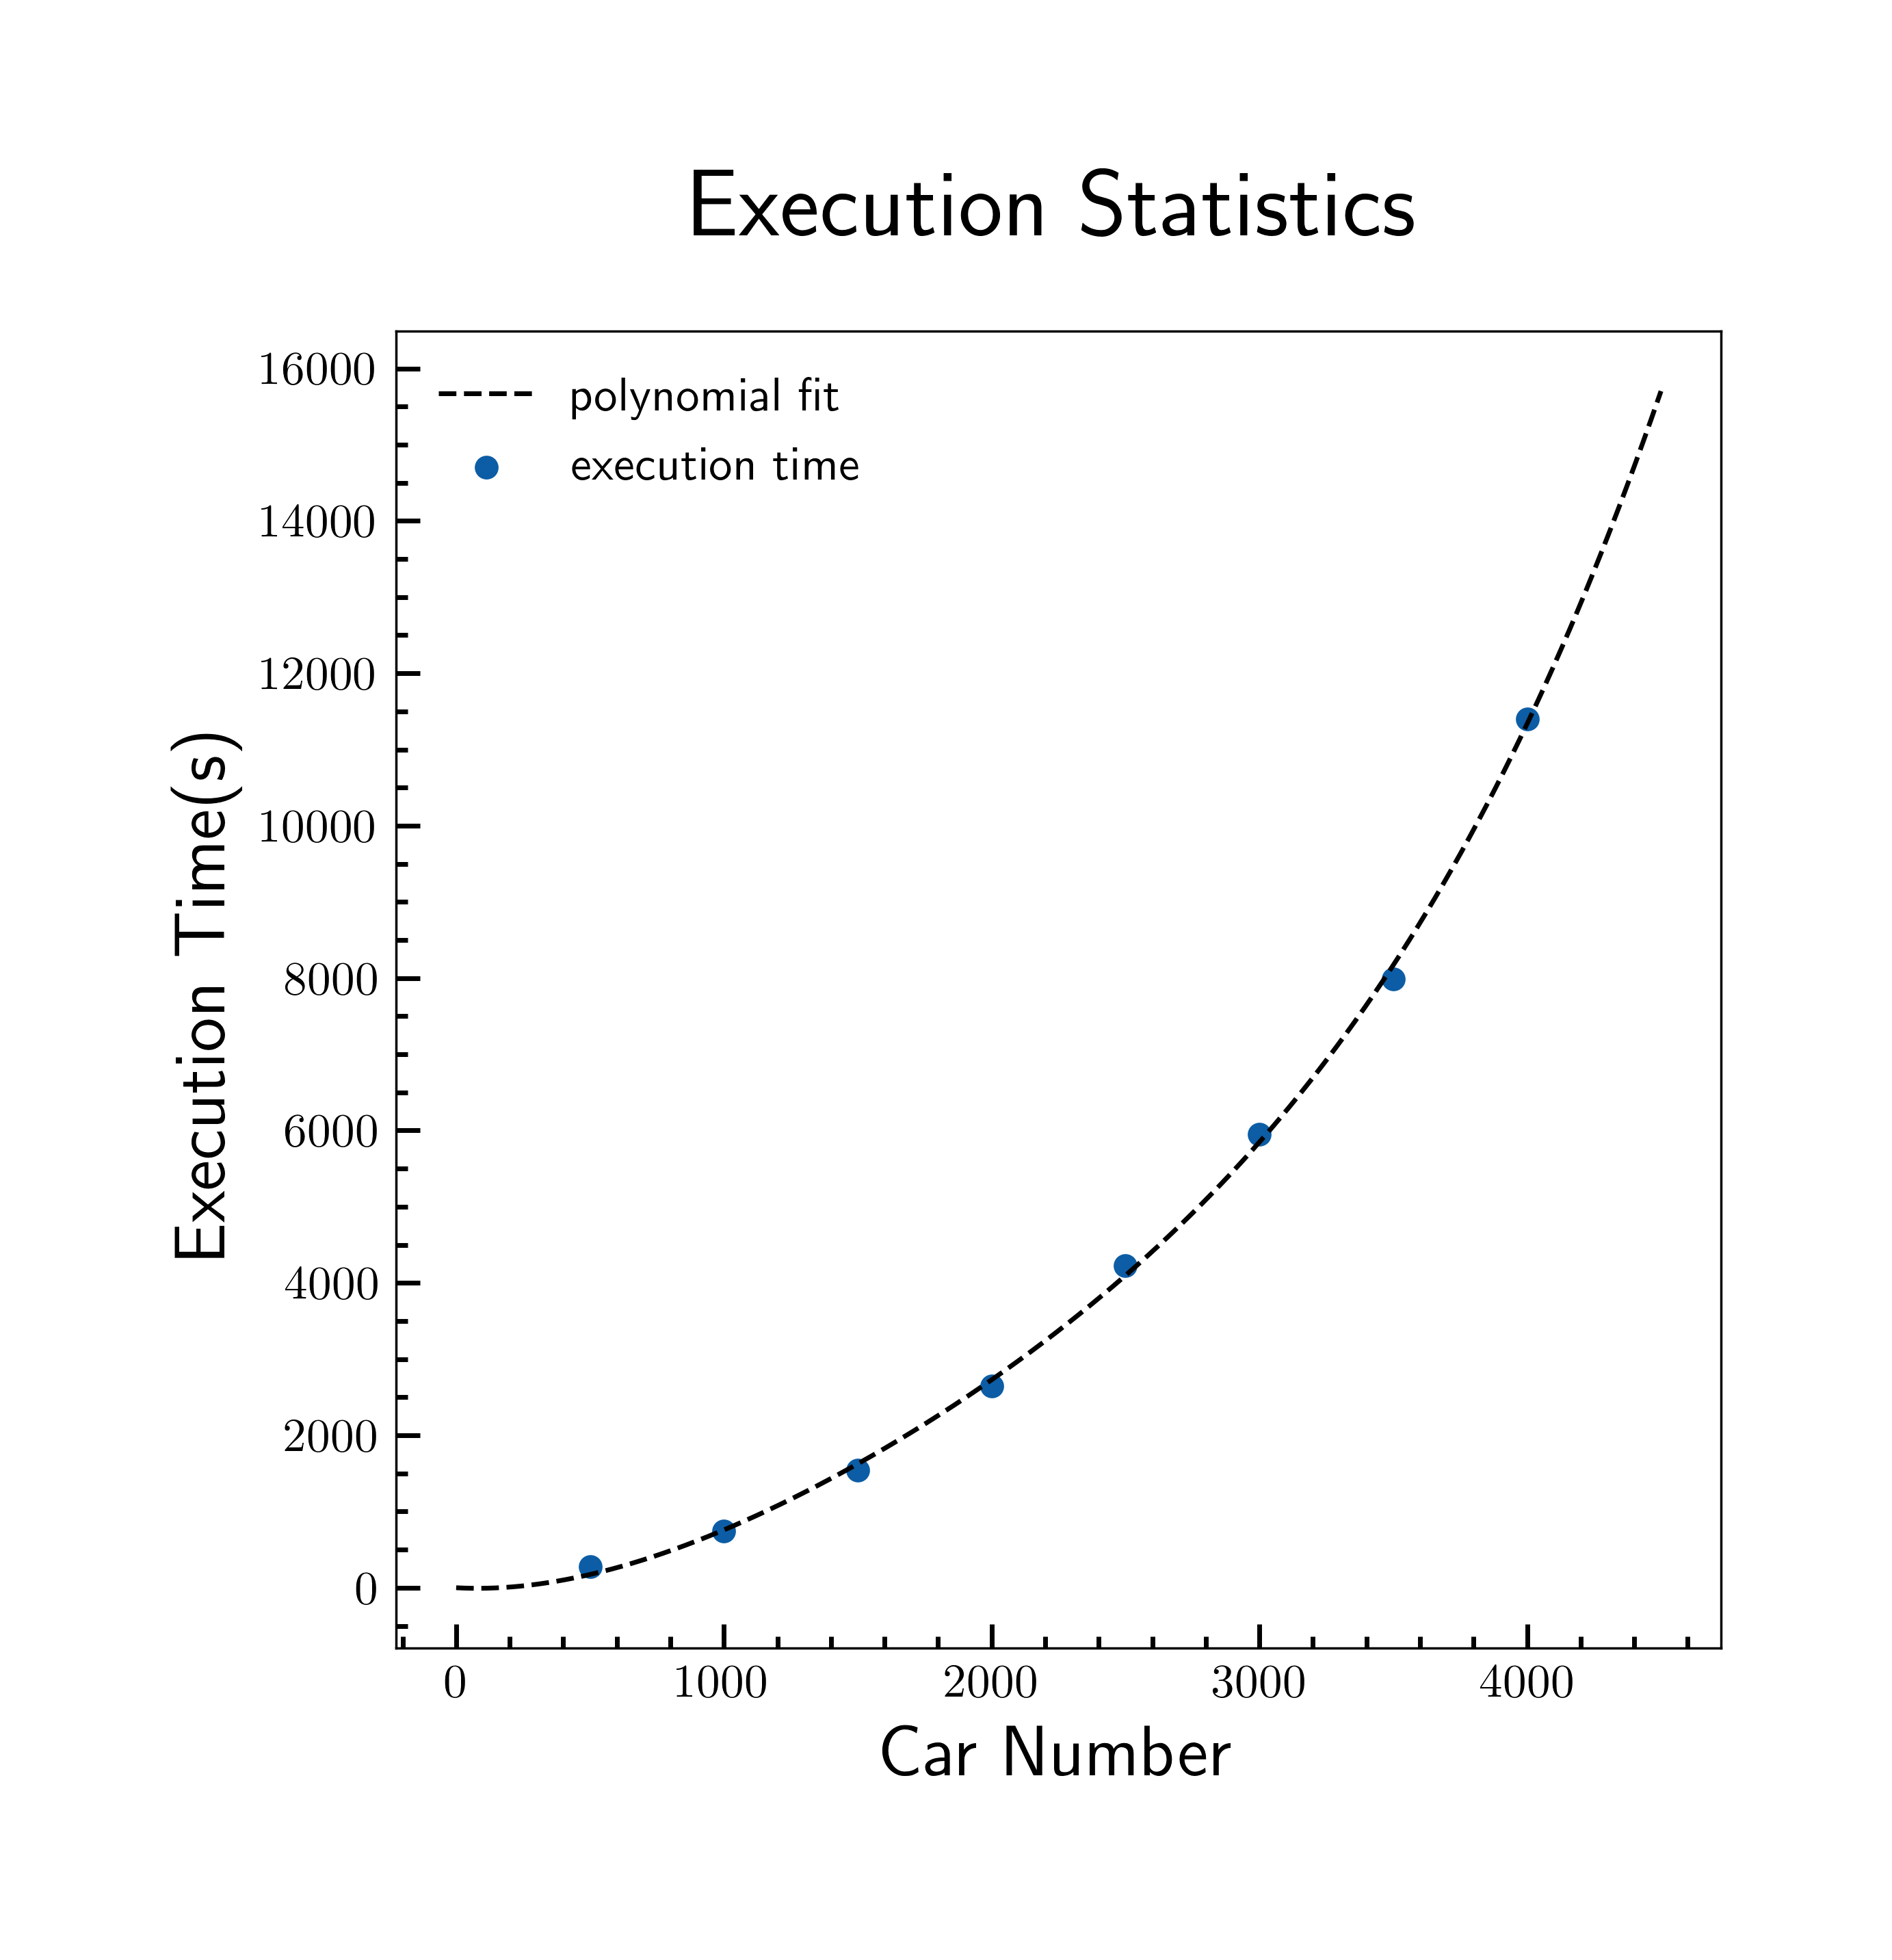
\includegraphics[width=9cm, height=9cm]{execution_time.png}
            \caption{Tempo di esecuzione di oneway increment simulation al variare del numero di auto generate.}
            \label{fig:10}
        \end{figure}

        Tale analisi dà un' idea di come il numero di iterazioni necessarie a portare le auto a destinazione non cresca linearmente come sarebbe in una città ideale,
        e tale effetto è dovuto all'emergere del traffico.

        \subsection{Considerazioni}

        Da tali risultati non possiamo dire che in alcuni casi convenga mettere sensi unici a più corsie piuttosto che sensi alternati,
        tuttavia i risultati suggeriscono l'emergenza del traffico all'aumentare della densità, che è necessario per stabilire la correttezza del 
        nostro modello. Inoltre è verificato il limite ideale, ovvero che per un numero di auto tendente a zero l'indice di traffico tende a 1, e 
        questo ci dà un'ulteriore dato a favore del corretto funzionamento del modello. Gli effetti ricercati possono essere stati nascosti da 
        varie caratteristiche del nostro modello, tali caratteristiche sono discusse nella conclusione.

    
\end{document}